%\documentclass[12pt,a4paper,twoside]{book} 
\usepackage[spanish]{babel} % de pedro
\usepackage{graphics,graphicx,epsfig,color,float,afterpage,fancyheadings,subfigure,moreverb,alltt} % de pedro
\usepackage[latin1]{inputenc} % tildes de pedro

\usepackage{algorithm}
\usepackage{algorithmic}

\usepackage{rotating}
\usepackage{url}

%% Esta letra se convierte mejor a pdf que la normal
\usepackage{ae}

%%% Para las fuentes matemticas
\usepackage{amsfonts}

\usepackage{subfigure}

\usepackage{pstricks} % para los dibujos del da
\usepackage{lscape} % para las pginas en horizontal
\usepackage{portland} % para las pginas en horizontal
\usepackage{supertabular} % para las tablas de ms de una pgina
\usepackage{tabularx} % para las tablas del tipo tabularx
%\usepackage{glossary}
%\documentclass[a4paper,spanish,12pt]{book} % esto es de gustavo
%\usepackage{amsmath,amsfonts}   % underset mathbb
%\usepackage{authordate1-4}      % bib style
%\usepackage{epsfig}     % eps
\usepackage{epic}           % graficos
%\usepackage{eepic}           % graficos
\usepackage{curvesls}           % curvas
\usepackage{amssymb}
%\usepackage{fancyheadings}  % encabezados
%\usepackage{hhline}             % hhline
%\usepackage[latin1]{inputenc}   % tildes
%\usepackage{makeidx}        % ndices
%\usepackage{setspace}           % interlinea
%\usepackage[spanish]{babel} % espaol

%%%%%%%%%%%%%%%%%%%%%%%%%%%%%%%%%%%%%%%%%%%%%%%%%%%%%%%%%%%%%%%%%%%%%%%%%%%%%%%

\author{juanlu}
\title{Tesis de Juan Lus Jimnez Laredo}




\newcommand{\fecha}{\footnotesize{[ Impreso: \the\day-\ifcase\month\or
    Ene\or Feb\or Mar\or Abr\or May\or Jun\or Jul\or Ago\or Sep\or
      Oct\or Nov\or Dic\fi-\the\year ]}}

\newcommand{\N}{\mathbb{N}}

%% Para corregir las cabeceras largas
\newcommand{\cabecera}[2]{
\markright{\ref{#1}. \hspace{0.1ex} \MakeUppercase{#2}}}


%\pagestyle{headings}
%\renewcommand{\chaptermark}[1]{\markboth{\fecha \\ \\ #1}{}}
%\renewcommand{\sectionmark}[1]{\markright{#1 \\ \\ \fecha}}
%\addtolength{\headheight}{2.5pt}



%\lhead[\it\thechapter]{\sl\rightmark}
%\rhead[\rm\leftmark]{\it\thesection}
%\rfoot[]{\thepage}
%\cfoot[]{}
%\lfoot[\thepage]{}

%\thispagestyle{plain}

\setcounter{secnumdepth}{3}
\setcounter{tocdepth}{3}

%\renewcommand{\baselinestretch}{1.2}
%\setlength{\parskip}{0.8ex}

\newtheorem{theorem}{\sf Teorema}
\newtheorem{lemma}{\sf Lema}

\newcommand{\rem}[1]{\S\iffalse #1 \fi}
\newcommand{\cur}[1]{ {\it #1\/} }
\newcommand{\crcl}[1]{#1\kern-9pt\raise1pt\hbox{$\bigcirc$}}
\newcommand{\evag}{{\sf EvAg}}
\newcommand{\evagp}{{\sf EvAg.}}
\newcommand{\evags}{{\sf EvAgs}}
\newcommand{\evagsp}{{\sf EvAgs.}}

\newcommand{\prog}[2] {
   \small
   \begin{minipage}[t]{75mm} {\tt #1}  \end{minipage}
   \begin{minipage}[t]{60mm} {#2}      \end{minipage}
   \\
}
\newcommand{\prg}[2] { {\tt #1} & {\sf #2} \\}

\newcommand{\wmfspecial}[4]{
   \begin{figure}[h]
   \centerline{\psfig{figure=#1,height=#2}}
   \caption{#3}   \label{#4}
   \end{figure}
}                   % USO: \wmfspecial{nombre.eps}{altura}{leyenda}{etiqueta}

\def\stackunder#1#2{\mathrel{\mathop{#2}\limits_{#1}}}

\def\marco #1#2#3#4{\centerline{       % USO: \marco{.1}{10}{124mm}
  \vbox{\hrule height #1pt%
  \hbox{\vrule width #1pt\kern #2pt%
  \vbox{\kern #2pt%
  \vbox{\hsize #3\noindent #4}%
  \kern #2pt}%
  \kern #2pt\vrule width #1pt}%
  \hrule height0pt depth #1pt}} }


\newcommand{\symnote}[2]{\symbolnote{#1}{#2}}

\newfont{\bi}{cmbxti10 scaled\magstep1}       % bf + it


%% Ruta de las figuras
\graphicspath{{../figuras/}}


\begin{document}
           % Eliminarlo al compilar el documento maestro, ponerlo para compilarlo separado

%%%%%%%%%%%%%%%%%%%%%%%%%%%%%%%%%%%%%%%%%%%%%%%%%%%%%%%%%%%%%%%%%%%%%%%%%%%%%%%
%%                                                                           %%
%%                             Tesis Doctoral:                               %%
%%                         Juan Luis Jimenez Laredo                          %%
%%%%%%%%%%%%%%%%%%%%%%%%%%%%%%%%%%%%%%%%%%%%%%%%%%%%%%%%%%%%%%%%%%%%%%%%%%%%%%%
\appendix
\cabecera{cap:appendixA}{Appendix A: Tuning of the Cache size parameter }
\chapter{\textit{Tuning of the Cache size parameter}}
\label{cap:appendixA}
\cabecera{cap:appendixA}{Appendix A: Tuning of the Cache size parameter }



Parallelising an EA implies the use of new parameters to control issues such as migration rates or the topology management. These new components drastically increase the complexity for the fine-tuning of the algorithm. In this sense, Cant\'u-Paz in \cite{cantu99:topologies} and Hidalgo and Fernandez in \cite{Fernandez:balancing} analyse up to seven  parameters derived from the parallelisation using islands. Within the \evag model instead, newscast simplifies all the decision making for the parallelisation by tuning  a single parameter, the cache size. The cache acts as a routing table  in which every peer holds a list of neighbours peers. Therefore, the cache size represents the maximum number of connections (edges) that a peer could have. Taking into account the recommendations of Jelasity et al. in \cite{jelasity:gossip}, the cache size has to be much smaller than the number of peers in order to get small-world features such as a small network diameter or a high clustering coefficient. 

Given the importance of the parameter, this appendix tries to calibrate an adequate cache size for the problems under study in this thesis. To this aim, we  measure the influence of different cache and population sizes on the algorithm performance when tackling a 4-trap instance. As will be shown, results indicate that success rates of the algorithm remain constant independently of the different cache sizes. This fact points to the robustness of the parallel model and helps decision making. Any cache size guaranteeing a small-world topology will produce equivalent performances.

Table \ref{table:appendix:parameters} summarizes the settings for the experiments in which eleven different cache sizes and two different population sizes have been tested.




\begin{table}[htbp]
\centering
{\scriptsize
\begin{tabular}{r c}
\hline
\multicolumn{2}{l}{\textbf{Problem instance}}\\
\hline
Problem & 4-trap\\
Chromosome length & 36\\
\\
\multicolumn{2}{l}{\textbf{\evag settings}}\\
\hline
Population size & 400, 600 individuals \\
Selection & Binary Tournament\\
Recombination & Uniform Crossover, $p_c = 1.0$ \\
Max. Eval. & 500000\\
\\
\multicolumn{2}{l}{\textbf{Newscast settings}}\\
\hline
 $Cache_{size}$ & 10,14,18,22,26,30,34,38,42,46,50\\ 

\end{tabular}
}
\caption{Settings for the experiments.\label{table:appendix:parameters}}
\end{table}




%%%%%%%%%%%%%%%%%%%%%%%%%%%%%%%%%%%%%%%%%%%%%%%%%%%%%%%%%%%%%%
\section{Analysis of Results}

Figure \ref{fig:cache:4trap} shows the SR and AES of the \evag 
model when tackling the 4-trap instance using different cache and population sizes. It can be observed how the population size has an impact on the algorithm performance while the cache size does not. 

The P2P EA is sensitive to the population size since the algorithm converges with a SR $\sim 0.85$ for $N=600$ while it decreases to $\sim 0.52$ for $N=400$. Nevertheless, results for different cache sizes move around the same SRs and AES. This way, neither the algorithm quality nor the execution time seems to be altered when using different settings for the cache size.

%The larger population size improves the quality of the solutions increasing, in turn, the computational effort. However, the cache size parameter does not seem to alter the algorithm performance neither in terms of quality (SR) nor execution-times (AES).

  

 This fact translates into the robustness of the \evag model with respect to such a parameter and is specially remarkable from the point of view of tuning the parameters of the algorithm. Choosing any cache size within the range $[10\dots50]$ will not alter the \evag performance.

\begin{figure}[htbp]
\centerline{
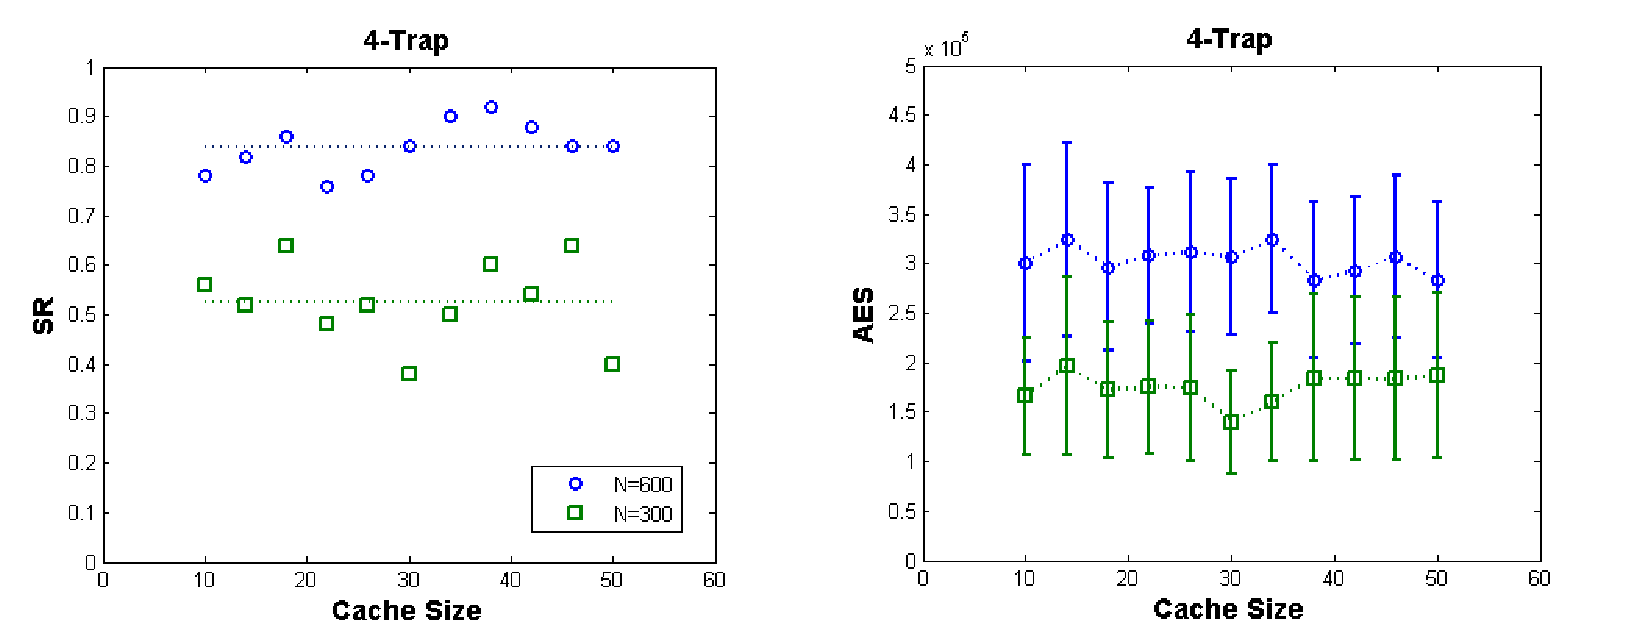
\includegraphics[width=\textwidth]{4trapcache}
}
\caption{Success Rate of the \evag model ({\em left}) and Average Evaluation to Solution with standard deviation ({\em right})
for a 4-trap instance using population sizes of $N=400$ and $N=600$. Averaged values for the different cache sizes in dotted lines.}
\label{fig:cache:4trap}
\end{figure}





%\bibliographystyle{alpha}  % Eliminarlo al compilar el documento maestro, ponerlo para compilarlo separado
%\bibliography{evagperformance,pea,p2pcomputing,model}% Eliminarlo al compilar el documento maestro, ponerlo para compilarlo separado

%\end{document}             % Eliminarlo al compilar el documento maestro, ponerlo para compilarlo separado
